%第3章
%図をすべて変更する必要があり

\section{詳細設計}

本節では感染症予防サポートシステムにおける詳細な動作,詳細設計について述べる.

まず,オブジェクト間のメッセージのやりとりを中心に,詳細な動作をシーケンス図を用いて説明する.
「室内状況を監視する」シーケンス図を図\ref{seq_kanshi}に,
「入室危険度の確認」のシーケンス図を図\ref{seq_enterlisk}に,
「換気要請の受け取り」のシーケンス図を図\ref{seq_kanki}に,
「室内環境状態の表示」のシーケンス図を図\ref{seq_kankyou}に示す.
\begin{figure}[htbp]
    \centering
    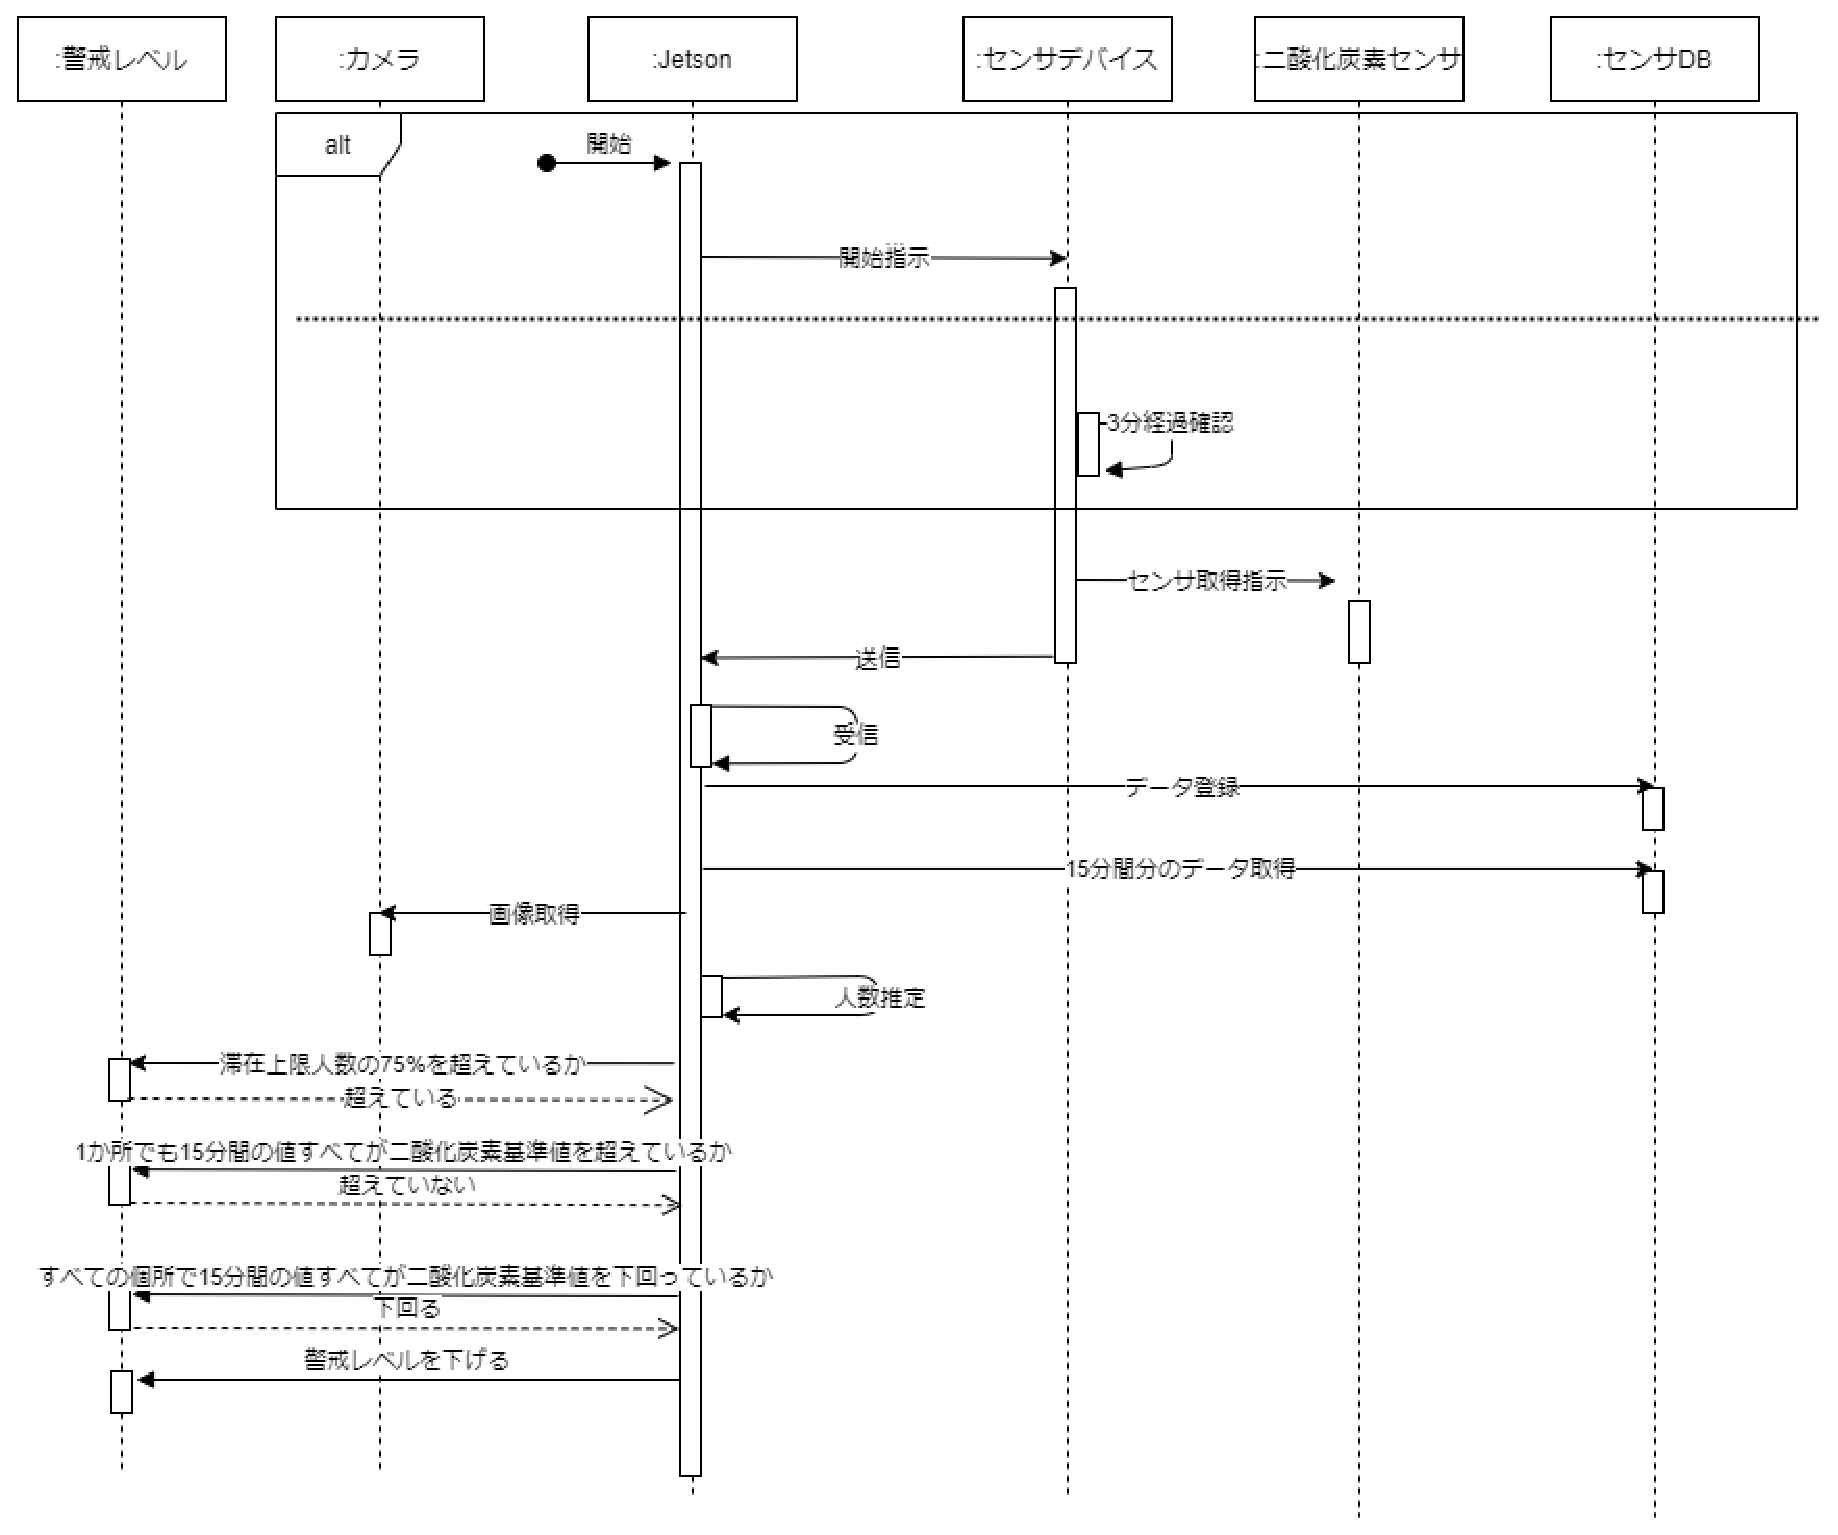
\includegraphics[width = 15cm]{./picture/sequence_kanshi_3.eps}
    \caption{ユースケース「室内状況を監視する」のシーケンス図}
    \label{seq_kanshi}
\end{figure}
\begin{figure}[htbp]
    \centering
    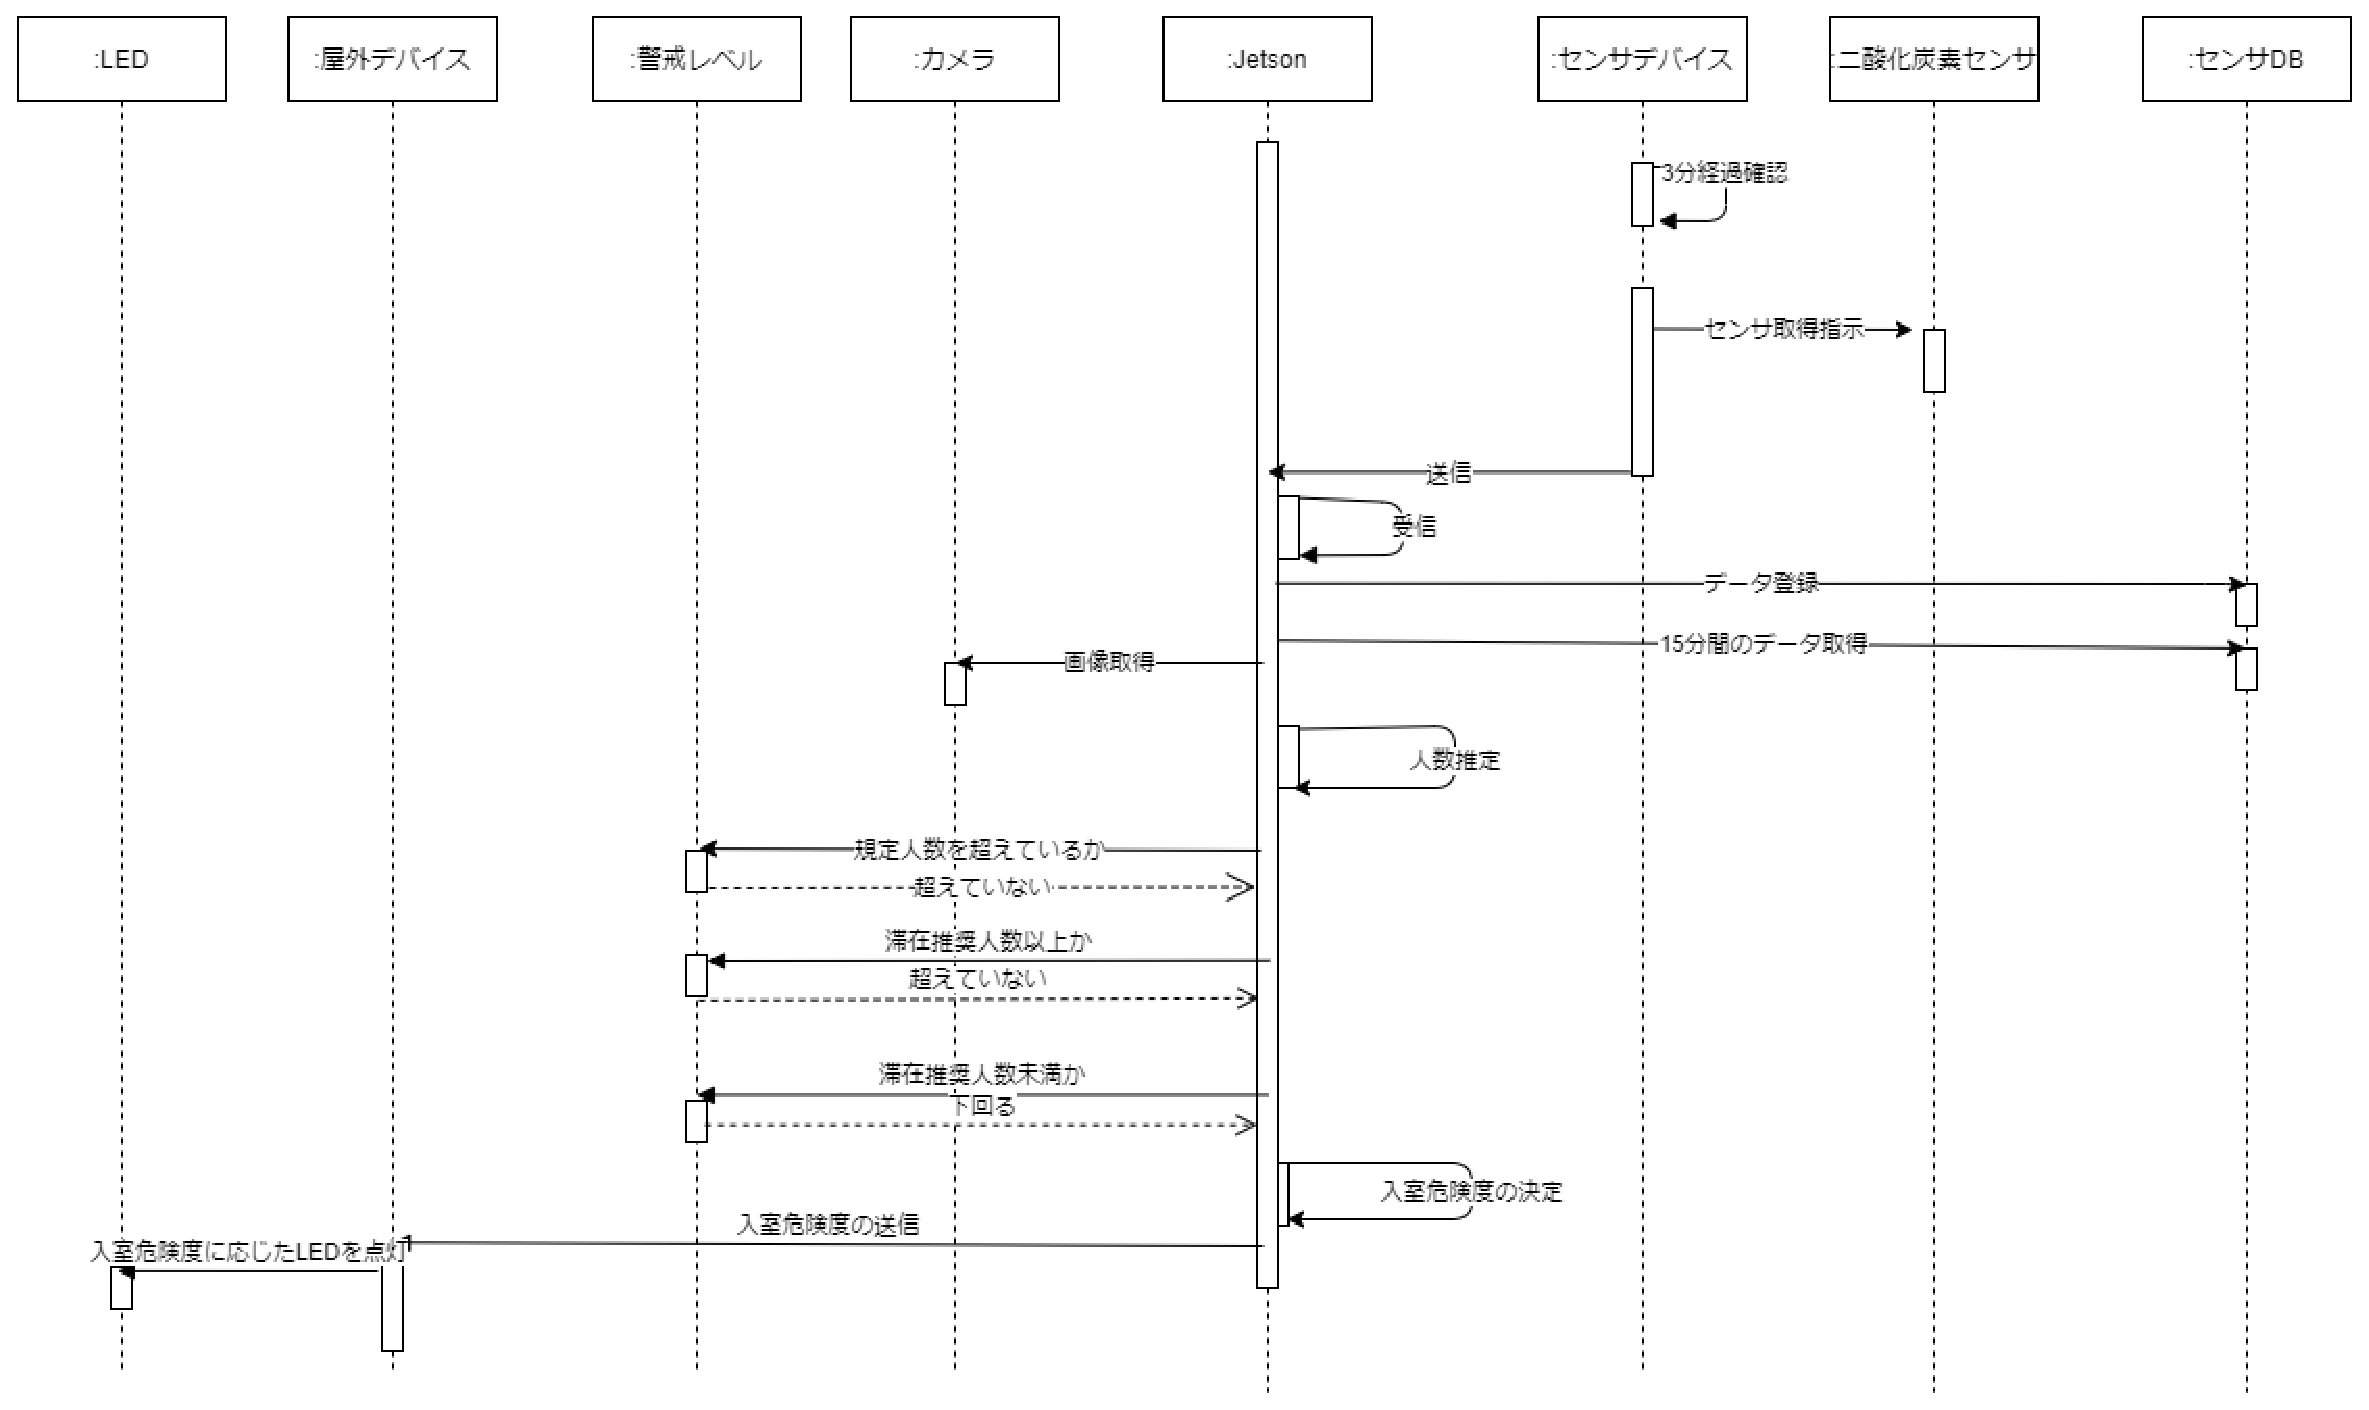
\includegraphics[width = 15cm]{./picture/sequence_nyushitsu_2.eps}
    \caption{ユースケース「入室危険度の確認」のシーケンス図}
    \label{seq_enterlisk}
\end{figure}
\begin{figure}[htbp]
    \centering
    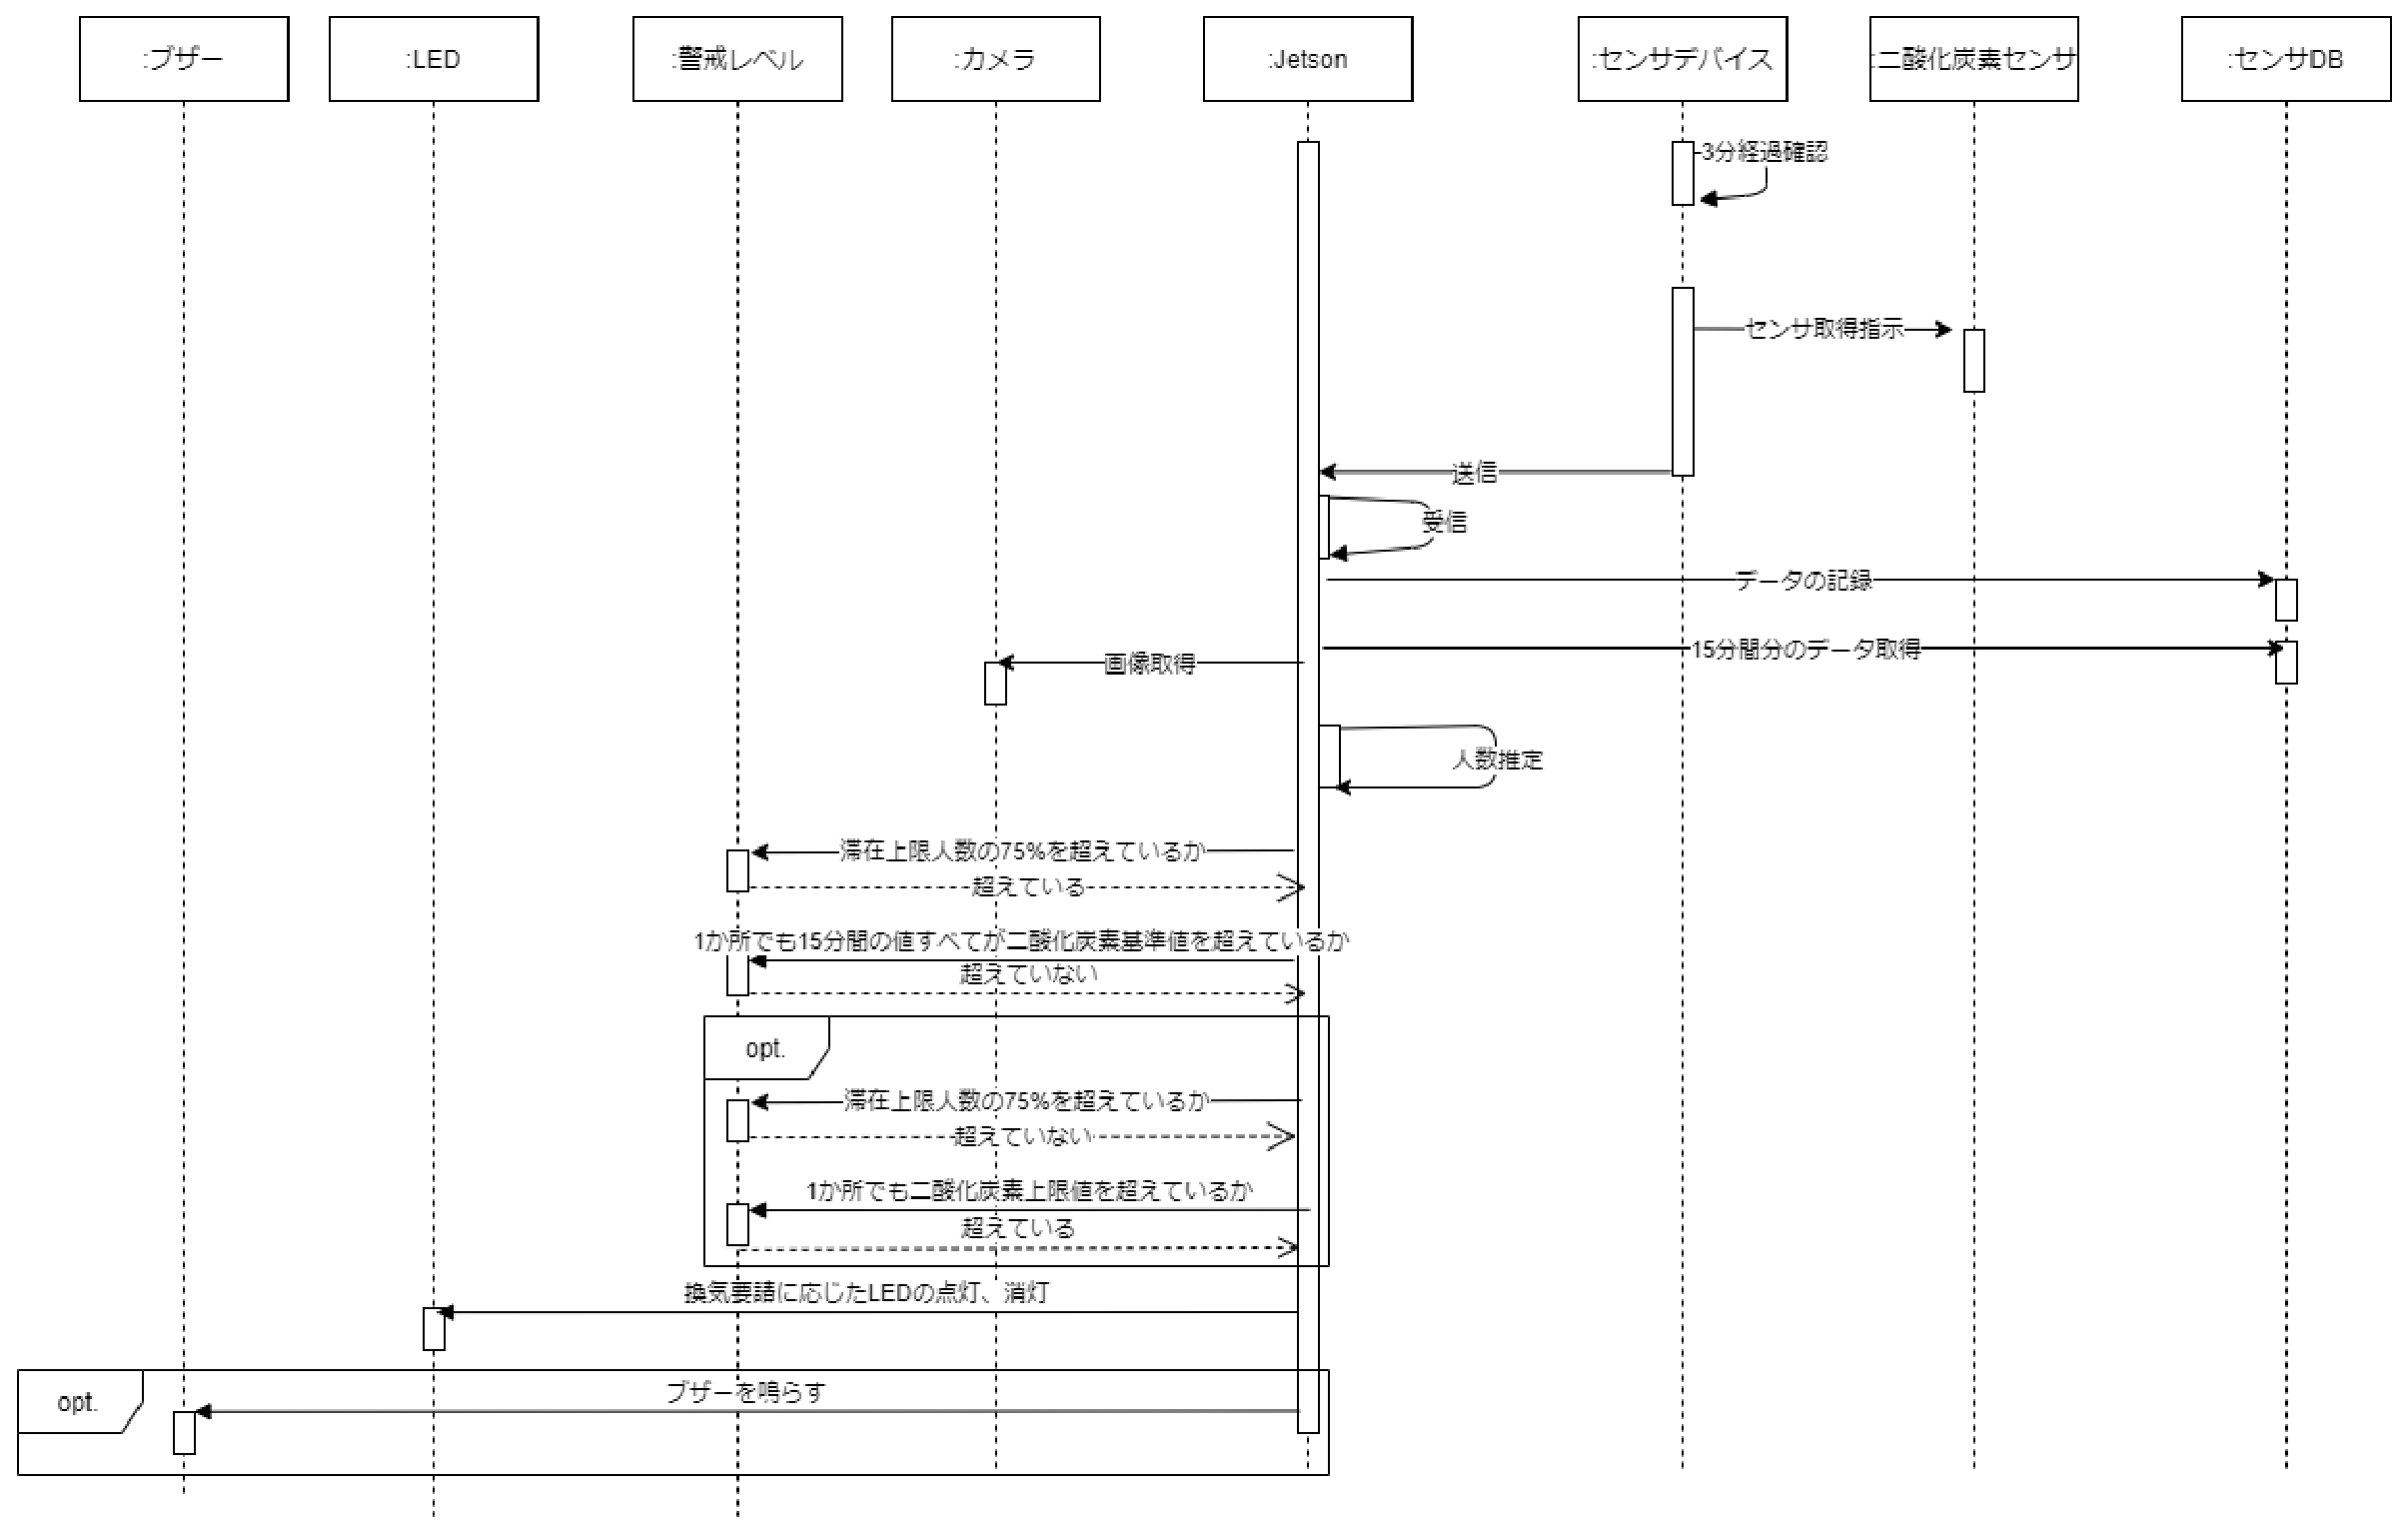
\includegraphics[width = 15cm]{./picture/sequence_kanki_2.eps}
    \caption{ユースケース「換気要請の受け取り」のシーケンス図}
    \label{seq_kanki}
\end{figure}
\begin{figure}[htbp]
    \centering
    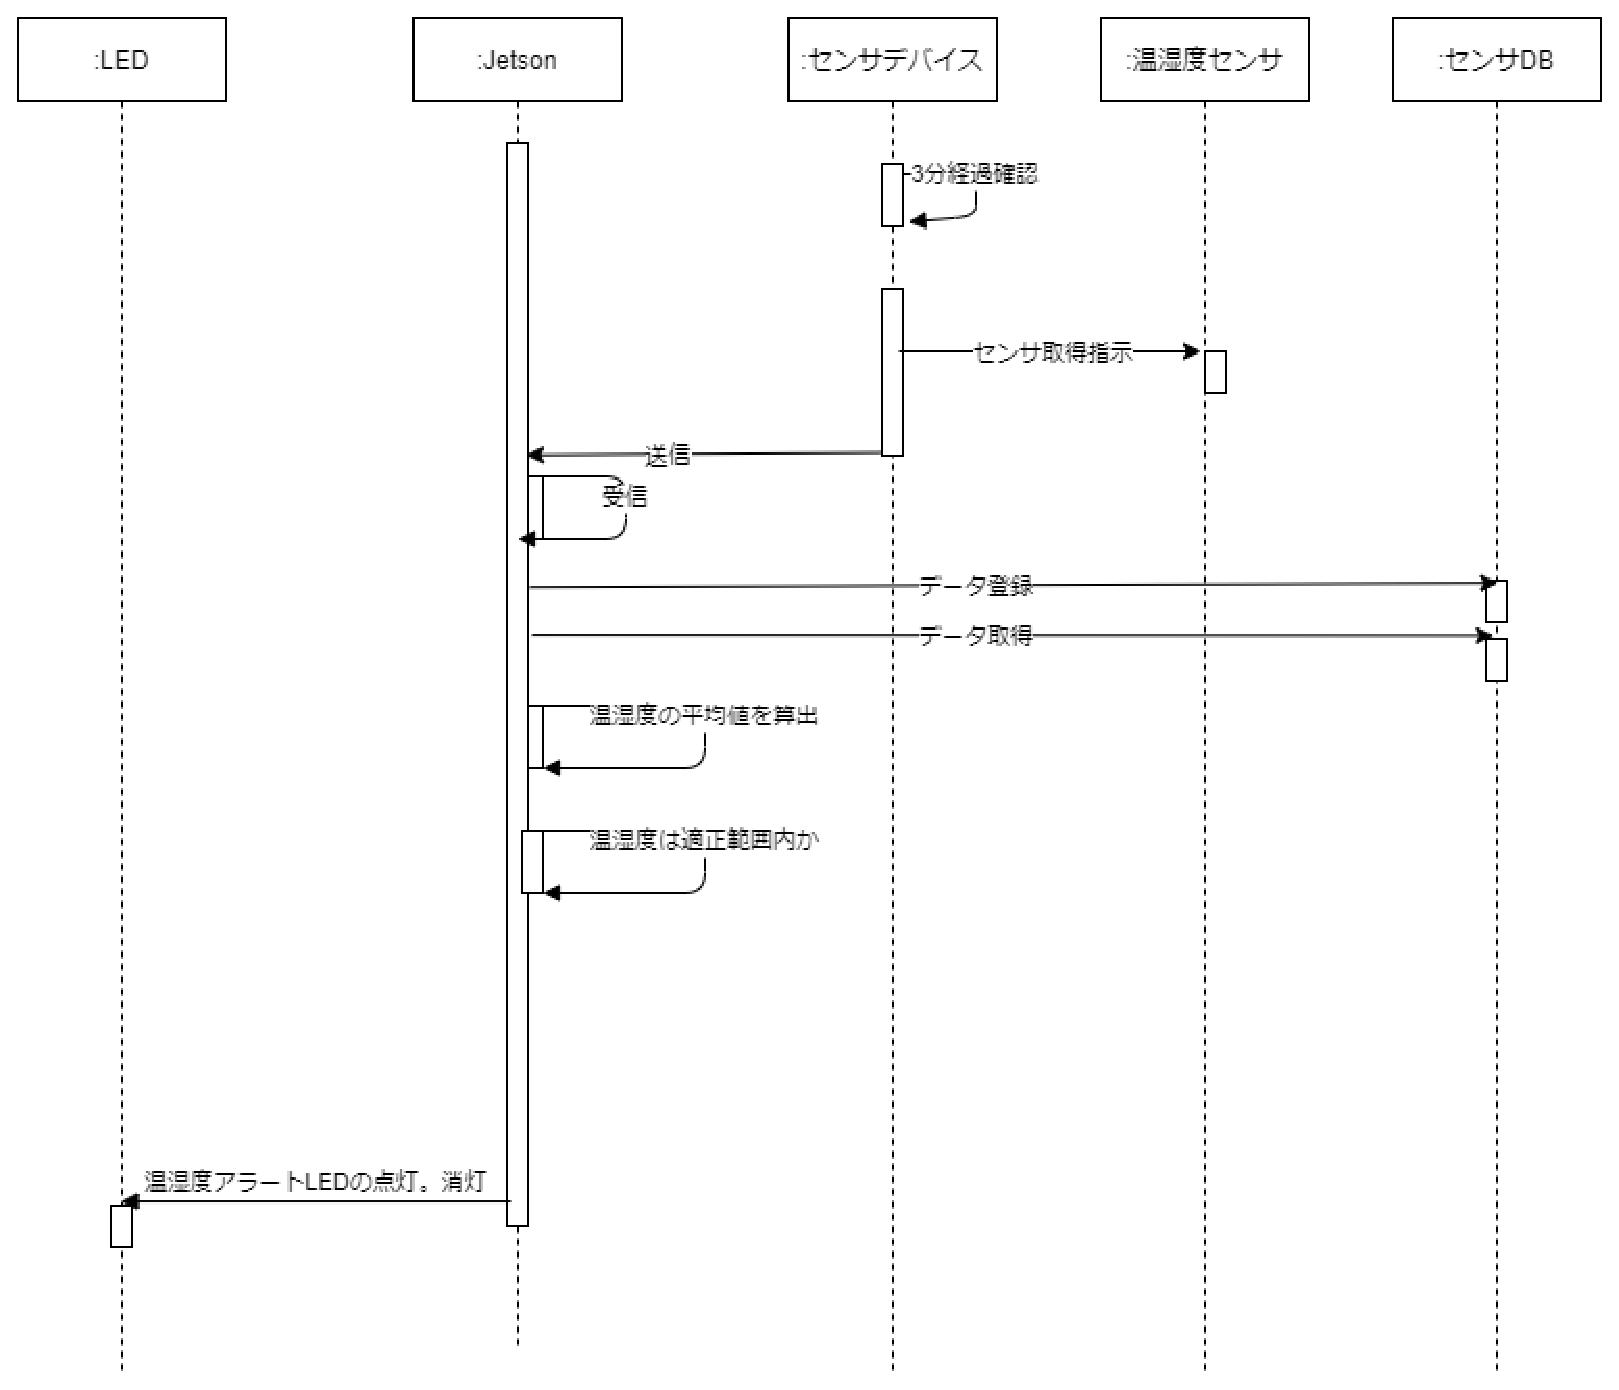
\includegraphics[width = 15cm]{./picture/sequence_shitsunai_2.eps}
    \caption{ユースケース「室内環境状態の表示」のシーケンス図}
    \label{seq_kankyou}
\end{figure}

まず,「室内状況を監視する」際の動作を説明する.
まず,システムが起動され,監視が開始した時には,Jetsonがセンサデバイスに対して開始指示を発する.
それを受け,センサデバイスはセンサからの値取得を行い,Jetsonに送信する.
また,システムが開始された時以外にも,センサデバイスが直近の値取得から3分経過を確認した場合であっても,センサの値取得を行う.
なお,この際送信されるデータは二酸化炭素濃度,温湿度,およびセンサデバイスの識別子である.
Jetsonで受信したデータは,センサDBに登録する.
その後,JetsonはセンサDBより直近15分間分のデータを取り出し,人数推定,および警戒レベルの調整を行う.
受信については,Jetson上で他の処理とは独立したスレッドで行い,受信漏れが起こらないようにする.
スレッド間でのデータのやり取り,および15分間分過去にさかのぼったデータ取得を容易にするため,データの保管にはセンサDBを使用した.
なお,基準値との比較方法について,基準値を上回っているかどうかは,複数あるセンサデバイスのうち一台でも連続して上回っているものがあれば超えているとみなす.
一方,基準値を下回っているかどうかは,複数あるセンサデバイスのすべてが連続して基準値を下回っているかどうかによって判断する.
なお,図\ref{seq_kanshi}では,例として警戒レベルを下げる際の処理の流れを示している.
ほかの場合の処理については,図\ref{act_kanshi}で示した条件に従い,同様に処理が行われる.
また,あらかじめ指定された時間になると監視を一時停止し,再度システムを起動する.
これは消費電力を抑えるために,夜間などの部屋があまり利用されない時間はシステムを停止させるものである.
一時停止したのち,復帰時間になると,再度監視を開始し,センサデバイスへの開始指示から行うこととした.

続いて,「入室危険度の確認」を行う際の動作を説明する.
センサの値を取得し,人数推定を行うまでは上記「室内状況を監視する」場合と同じである.
その後,警戒レベルが保有している規定人数,および滞在推奨人数との比較を行い,その結果をもとにJetsonが入室危険度の判定を行う.
入室危険度は,そのまま屋外デバイスに通知され,屋外デバイスはそれを受けてLEDを点灯させる.
なお,図\ref{seq_enterlisk}では,一例として入室危険度が「青」と判断される場合の動作を示している.
ほかの場合の処理については,図\ref{act_enterlisk}で示した条件に従い,同様に処理が行われる.

次に,「換気要請の受け取り」を行う際の動作を説明する.
センサの値を取得し,人数推定を行うまでは上記「室内状況を監視する」場合と同じである.
その後,警戒レベルが保有している二酸化炭素濃度の基準値と定められている滞在上限人数とをもとに比較し,換気要請の判断を行う.
二酸化炭素濃度の基準値が超えているかどうかは複数あるセンサデバイスのうち,一台でも連続して値が超えているものが存在すれば超えているものとして判断をする.
その後,LEDを光らせる際には,Jetsonから直接接続したLEDの点灯を行い,点灯する場合は同時にブザーも鳴らす.
なお,図\ref{seq_kanki}では,換気要請を行う場合と換気要請を行わない場合の一例の流れを示している.
他の場合の処理については,図\ref{act_kanki}で示した条件に従い,同様に処理が行われる.

最後に,「室内環境状態の表示」を行う際の動作を説明する.
センサの値を取得するまでの動作は上記「室内状況を監視する」場合と同じである.
その後,センサDBより,その時に取得された全センサデバイスの温湿度の値を読み出し,温度,湿度の平均値を求め,それを代表値とする.
その代表値が適正範囲内にあるかどうかを判断し,範囲外であった場合は,Jetsonに接続されているLEDを点灯する.
温湿度が範囲内であった場合にはLEDを消灯させる.
%なお,本システム湿度30\%以上を適正範囲として制定し,温度については定めないこととした.

続いて,私が担当したセンサデバイスの状態遷移について,ステートチャート図を用いて説明する.
センサデバイスのステートチャート図を図\ref{state_sensor}に示す.
\begin{figure}[htbp]
    \centering
    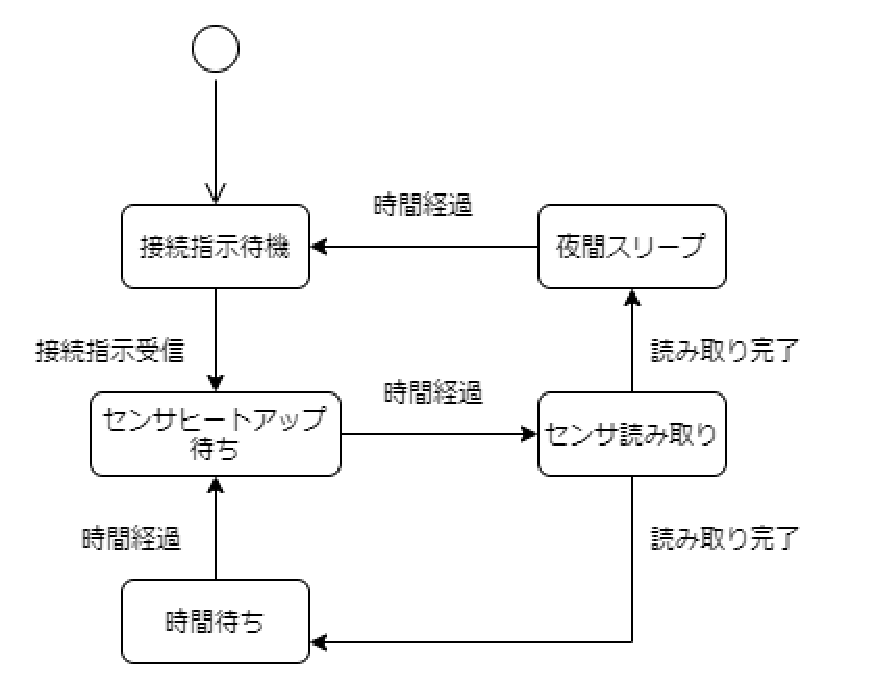
\includegraphics[width = 9cm]{./picture/statechart_micon.eps}
    \caption{センサデバイスのステートチャート図}
    \label{state_sensor}
\end{figure}
センサデバイスの状態は「接続指示待機」,「センサヒートアップ待ち」,「時間待ち」,「夜間スリープ」,「センサ読み取り」の5状態を持つとした.
まず,センサデバイスの電源を入れることで,初期状態の「接続指示待機」状態となる.
この状態では,システムを開始した際,開始指示を受信するまで待機するものである.
その後,「センサヒートアップ待ち」状態へと推移する.
これは,本システムで使用する二酸化炭素濃度センサが,通電直後の場合,正しい値を示さない可能性があり,ヒートアップ時間を必要とするため,その時間を確保するものである.
この間は,マイコンボード,および昇圧センサを介して二酸化炭素濃度センサに電力供給を行う.
なお,この際,センサデバイスが起動している,および受信待機状態であることを確認できるようにするため,この状態のときにはセンサデバイスに接続したLEDを点滅させるようにした.
その後,ヒートアップ時間が経過すると温湿度,二酸化炭素センサの読み取りとJetsonへの送信を行う「センサ読み取り」状態に推移する.
センサの読み取りと送信が終了すると「時間待ち」状態に推移する.
「時間待ち」状態は,二酸化炭素センサへの給電は行わず,できるだけ消費電力を抑えた状態である.
3分毎に値を読み取るので,3分から二酸化炭素センサのヒートアップに要する時間を引いた時間だけこの状態を保つ.
その後,「センサヒートアップ待ち」状態へと戻り,繰り返される.
最後に,あらかじめ指定された時間になると「センサ読み取り」状態からセンサ読み取り,Jetsonへの送信を行ったのち,「夜間スリープ」状態へと推移する.
これは,動作としては「時間待ち」状態と同じく,省電力状態で待つものであるが,これは部屋の利用が少ない時間に推移する状態である.
従って,「時間待ち」状態よりも長い間,この状態を保つことになる.
その後は,マイコンボード内とJetson内のタイマーがずれてしまうことが考えられるため,「接続指示待機」状態へと推移する.
夜間スリープ状態から推移するのは1日に一度であるので,その際に再度接続指示を受け,Jetsonとセンサデバイスの開始時間を1日ごとに同期する狙いがある.
また,「接続指示待機」以外の状態においては,電池の交換時期が分かるよう,供給電力が低くなった際に,センサデバイスに接続したLEDを点灯させることとした.

これらの設計を受け,表\ref{twelite_test_koumoku}の通り,センサデバイスにおける単体テストの項目をデバイスごとに制定した.
\begin{table}[htbp]
    \centering
    \caption{センサデバイスにおける単体テスト項目}
    \label{twelite_test_koumoku}
    \includegraphics[width = 15cm]{./picture/tantaitest_twelite_koumoku.eps}
\end{table}
なお,消費電力化の目安として,部屋の使用時間が12時間とした際,起動してから最初の「夜間スリープ」状態への遷移が行われるまでは乾電池交換を行うことなく動作できることが最低限必要であるとした.


% オブジェクト間のメッセージのやりとりを時系列に沿って表現するために,シーケンス図を作成した.図\ref{sequence_ic}に,ICタグを用いた商品識別システムのシーケンス図を示す.

% \begin{figure}[htbp]
% \centering
% \includegraphics[width=15cm]{./picture/sequence_ic.eps}
% \caption{ICタグを用いたシステムのシーケンス図}
% \label{sequence_ic}
% \end{figure}


% 図\ref{sequence_qr}はQRコードを用いたシステムのシーケンス図である.


% \begin{figure}[htbp]
% \centering
% \includegraphics[width=15cm]{./picture/sequence_qr.eps}
% \caption{QRコードを用いたシステムのシーケンス図}
% \label{sequence_qr}
% \end{figure}


% 図\ref{sequence_ic}と図\ref{sequence_qr}の違いはユーザ情報の登録の部分のみである.詳細設計まで行ったが,ICタグを用いたシステムとQRコードを用いたシステムの評価は3.2節から大きく変化しなかった.買い物と決済の設計においては共通しているため,そのまま優先度の高いシステムである下記の図\ref{sequence}部分を実装する.



% \begin{figure}[htbp]
% \centering
% \includegraphics[width=15cm]{./picture/sequence.eps}
% \caption{高優先度のシステムのシーケンス図}
% \label{sequence}
% \end{figure}


% 図\ref{sequence}において筆者の担当した部分はメッセージ2~6,10,11の部分である.各メッセージの詳細を下記に示す.


% \begin{quote}
% 2. 超音波センサ反応時にフラグをたてる.

% 3. フラグがたったら,0.5秒に一度,合計6枚の画像を撮り,データ送信用配列にデータを追加する.

% 4. 画像を撮ったことをユーザに知らせるためにLED緑を点灯させる.

% 5. ロードセルより重量が増加したか減少したかを確認し,増加の場合は追加として1,減少の場合は削除として2のフラグをたて,キューへフラグを追加する.ただし,±3gの増減は誤差とする.

% 6. 追加,削除のフラグが入っているキューを参照し,データ送信用配列にフラグ情報を追加し,画像データと合わせてサーバへ送信する.

% 10. バーコード情報を正しく読み取れたか,読み取れなかったかを知らせるフラグをサーバから受信する.

% 11. サーバがバーコード情報を正しく読み取ることができた場合はLED青を,正しく読み取ることができなかった場合はユーザに再度商品の追加,削除を促すためLED赤を点灯させる.
% \end{quote}

% なお,優先度の高い項目部分において,単体テストの際に用いる各センサのテスト項目を下記の表\ref{webcamera},表\ref{chouonpa},表\ref{rodoseru},表\ref{data}に示す.

% \begin{table}[htbp]
% \centering
% \caption{Webカメラの単体テスト項目}
% \includegraphics[width = 15cm]{./picture/webcamera.eps}
% \label{webcamera}
% \end{table}

% \begin{table}[htbp]
% \centering
% \caption{超音波センサの単体テスト項目}
% \includegraphics[width = 15cm]{./picture/chouonpa.eps}
% \label{chouonpa}
% \end{table}

% \begin{table}[htbp]
% \centering
% \caption{ロードセルの単体テスト項目}
% \includegraphics[width = 15cm]{./picture/rodoseru.eps}
% \label{rodoseru}
% \end{table}

% \begin{table}[htbp]
% \centering
% \caption{データ送信の単体テスト項目}
% \includegraphics[width = 15cm]{./picture/data.eps}
% \label{data}
% \end{table}.


%メッセージの説明